\chapter[WKB]{Introduction to WKB Theory}
Part VII of the course.
\begin{itemize}
	\item WKB theory is good for \underline{linear} ODEs and PDEs in which the highest derivative is multiplied by $\epsilon \ll 1$
	\item In the linear context, WKB subsumes the Boundary Layer (BL) theory
	\item \emph{But} the BL theory can also handle \underline{nonlinear} problems
	\item WKB theory is ideal for problems in which there's a \underline{global} (as opposed to a local) breakdown in the solution as $\epsilon \rightarrow 0^+$.  
	\item Arises often in quantum theory, acoustics, optics or other fields that deal with slowly-modulated waves or oscillations
\end{itemize}
 
\paragraph{Example 1:}
\begin{gather*}
	\epsilon y'' + y = 0 \\
	y(0) = 0 \qquad y(1) = 1
\end{gather*}
This is easily solved to yield
\begin{gather*}
	y(x,\epsilon) = \frac{\sin (x/\sqrt{\epsilon})}{\sin (1/\sqrt{\epsilon})} \qquad 
	\epsilon \neq \frac{1}{(n\pi)^2}
\end{gather*}
Note that as $\epsilon \rightarrow 0^+$, the solution $y(x,\epsilon)$ becomes more oscillatory over the whole domain -- there is no boundary layer. WKB handles problems like this.

\paragraph{WKB approximation}

We guess a solution of the form
\begin{gather*}
	y \sim \exp \left[\frac{1}{\delta} S(x)\right] \\
	S(x) = S_0 + \delta S_1 + \delta^2 S_2 + \dots 
\end{gather*}
with $\delta$ determined by dominant balance\footnote{Louiville and Greene introduced the $\me^{S(x)}$ move.}. For posterity we record the terms
\begin{align*}
	y' &\sim  \me^{S(x)/\delta }   \left[\frac{S'(x)}{\delta}\right]  \\
	 & \sim  \me^{S(x)/\delta } \left[\frac{S_0'}{\delta} + S_1' + \delta S_2' + \dots \right]  \\
	y'' &\sim  \me^{S(x)/\delta } \left[\frac{S''(x)}{\delta} + \frac{1}{\delta^2}\left(S'(x)\right)^2\right] \\
	& \sim \me^{S(x)/\delta } \left[ \frac{1}{\delta^2} (S_0')^2 + \frac{1}{\delta} (S_0'' + 2 S_0' S_1') + (S_1'' + (S_1')^2 + 2 S_0' S_2') + \dots\right]
\end{align*}


\paragraph{Example 2:} The ``Schr\"{o}dinger'' equation 
\begin{gather*}
	\epsilon^2 y'' = Q(x) y, \qquad\quad  0 < \epsilon \ll 1
\end{gather*}
is a broad class of second order ODE with the $y'(x)$ term absent. For now assume $Q(x) \neq 0$ for any $x$. Next proceed to substitute the WKB ansatz to write
\begin{align*}
	 \frac{\epsilon^2}{\delta^2} (S_0')^2 + \frac{\epsilon^2}{\delta} (S_0'' + 2 S_0' S_1') + \epsilon^2 (S_1'' + (S_1')^2 + 2 S_0' S_2') + \dots = Q(x)
\end{align*}
From dominant balance, setting $\delta = \epsilon$ gives us a nice hierarchy of equations:
\begin{align*}
	O(\epsilon^0):& \qquad (S_0')^2 = Q(x) \\
	O(\epsilon^1):& \qquad 2S_1'S_0' + S_0'' = 0 \\
	O(\epsilon^2):& \qquad 2S_2'S_0' + (S_1')^2 + S_1'' = 0 
\end{align*}
At the lowest order
\begin{align*}
	S_0' &= \pm \sqrt{Q(x)} \\
	\implies S_0 &= \pm \int_{a}^{x} \sqrt{Q(t)} \md t
\end{align*}
At the next order
\begin{align*}
	S_1' &= -\frac{1}{4} \frac{Q'(x)}{Q(x)} \\
	\implies S_1 &= -\frac{1}{4} \ln Q(x) + c
\end{align*}
Note that $Q(x) \neq 0$. Pulling these terms together
\begin{align}
	y(x,\epsilon) &\sim \exp \left[\frac{1}{\epsilon} S_0 + S_1 + O(\epsilon)\right] \nonumber\\
	& \sim \frac{1}{Q(x)^{1/4}} \left\{ c_1 \exp \left[\frac{1}{\epsilon} \int_{a}^{x} \sqrt{Q(t)}\md t \right]+ c_2 \exp \left[-\frac{1}{\epsilon} \int_{a}^{x} \sqrt{Q(t)}\md t \right] \right\} \label{eqn:wk18-wkb}
\end{align}
Since $\me^{\epsilon f } \approx 1 + \epsilon f + \dots $, the $O(\epsilon)$ terms may be neglected. 

\paragraph{Example 3:} 
\begin{gather*}
	\epsilon y'' + y' + y = 0 \\
	y(0) = 0 \qquad y(1) = 1
\end{gather*}
The BL theory provides the uniformly valid approximation 
\begin{gather*}
	y_c \sim \me^{1-x} - \me^{1-x/\epsilon} + O(\epsilon)
\end{gather*}
which has a BL near $x=0$. Here approach with the WKB method:
\begin{gather*}
	\epsilon \left[\frac{1}{\delta^2} (S_0')^2 + \frac{1}{\delta} (S_0'' + 2 S_0' S_1') + (S_1'' + (S_1')^2 + 2 S_0' S_2') + \dots\right] \\
	+ \left[\frac{1}{\delta}S_0' + S_1' + \delta S_2' + \dots \right] + 1 = 0
\end{gather*}
A consistent hierarchy of equations result when 
\begin{gather*}
	\frac{\epsilon}{\delta^2} \approx \frac{1}{\delta}
\end{gather*}
yielding
\begin{align*}
	O\left(\epsilon^{-1}\right):& \qquad  (S_0')^2 + S_0' = 0 \\
	O(\epsilon^0): & \qquad S_0'' + 2S_0'S_1' + S_1' + 1=0
\end{align*}
At the lowest order
\begin{align*}
	S_0'(S_0'+1) = 0 \qquad \implies 
	\begin{cases}
		S_0 = \text{const} \\
		S_0 = -x + \text{const}
	\end{cases} 
\end{align*}
The two cases would give us the two linearly independent solutions. At the next order
\begin{align*}
	\begin{cases}
		S_1 = -x + \text{const} \\
		S_1 = x + \text{const}
	\end{cases}
\end{align*}
Linearly combining the two solutions
\begin{align*}
	y(x,\epsilon) &\sim \exp \left[\frac{1}{\epsilon} S_0 + S_1 + \dots \right] \\
	&\sim c_1 \me^{-x} + c_2 \me^{- x/\epsilon + x}
\end{align*}
With the application of the BCs
\begin{align*}
	0 &= c_1 + c_2 \\
	1 &= c_1 \me^{-1} + c_2 \underbrace{\me^{-1/\epsilon + 1}}_\text{TST} 
\end{align*}
In the limit of $\epsilon \rightarrow 0^+$, $\me^{-1/\epsilon+1} \rightarrow 0$. This yields $c_1 = \me$, $c_2 = -\me$ and
\begin{align*}
	y(x,\epsilon) &\sim \me^{1-x} - \me^{1+x-x/\epsilon} \\
	& \sim \me^{1-x} - \me^{1-x/\epsilon} 
\end{align*}
Since outside the BL, $x=O(1)$ and the $x/\epsilon$ term dominates (the $\me^{1+x-x/\epsilon}$ term is a TST). In the BL, $x \leq O(\epsilon) \ll 1 $. From both arguments, the term $x$ can be ordered out and we end up with the identical BL solution. And yet, we did not have to do any matching in the overlap region. Therefore this is a \emph{global} method as opposed to a \emph{local} method in which we have to think about the BL.

\paragraph{Example 4:} The ``slowly aging spring''
\begin{gather}
	\ddot{x} + \underbrace{\me^{-\epsilon t}}_{k(t)} x = 0 \label{eqn:wk18-spring-eqn}
\end{gather}
Here, compared with Hooke's law, the mass is unity and the spring stiffness $k = k(t)$ decays very slowly. Observe that at very long times, specifically $t \gg 1/\epsilon$, $k(t) \approx 0$ and
\begin{gather*}
	x(t) = v t + \text{const}
\end{gather*}
That is, the oscillations are expected to stop. Let us introduce the slow time 
\begin{gather*}
	T = \epsilon t
\end{gather*} 
and rewrite our equation:
\begin{gather*}
	\epsilon^2 X'' + \me^{-T} X = 0
\end{gather*}
This is a Schr\"{o}dinger equation with $Q(T) = -\me^{-T}$. Using our earlier results
\begin{gather*}
	\epsilon^2\left[ \frac{1}{\delta^2} (S_0')^2 + \frac{1}{\delta} (S_0'' + 2 S_0' S_1') + (S_1'' + (S_1')^2 + 2 S_0' S_2') + \dots\right] + \me^{-T} = 0
\end{gather*}
The choice of $\delta = \epsilon$ gives us the consistent hierarchy 
\begin{align*}
	O(\epsilon^0): \qquad (S_0')^2 + \me^{-T} = 0 \\
	O(\epsilon^1): \qquad S_0'' + 2 S_0' S_1' = 0
\end{align*}
The first order solution is
\begin{align*}
	S_0' &= \pm \mi \me^{-T/2}\\
	\implies S_0 &= \mp 2\mi \me^{-T/2}
\end{align*}
At the next order
\begin{align*}
	S_1 = \frac{T}{4}
\end{align*}
Putting it all together
\begin{align}
	X(T) &\sim \exp\left[\frac{1}{\epsilon} S_0 + S_1 + \dots \right] \nonumber \\
	& \sim c_1 \exp\left[-\frac{2 \mi}{\epsilon}\me^{-T/2} + \frac{T}{4} + \dots \right] + c_2 \exp\left[+\frac{2 \mi}{\epsilon}\me^{-T/2} + \frac{T}{4} + \dots \right] \nonumber \\
	& \sim \me^{T/4} \left[a \sin \left(\frac{2}{\epsilon}\me^{-T/2}\right) + b \cos \left(\frac{2}{\epsilon}\me^{-T/2}\right)\right] \label{eqn:wk18-spring-wkb}
\end{align}
Note the following:
\begin{itemize}
	\item There is a slowly growing amplitude 
	\item It may be a good idea to define a nonlinear time $\tau = 2 \me^{-\epsilon t/2}/\epsilon$. In fact, under this transformation, the aging spring problem is exactly solvable in terms of the Bessel function!
\end{itemize}
The analytical and numerical results are compared subject to the conditions
\begin{gather}
	x(0)=1 \qquad x'(0)=0 \qquad \epsilon=0.05 \label{eqn:wk18-spring-ic}
\end{gather}
We solve for $a$ and $b$ using the equations
\begin{align*}
	a \sin (2/\epsilon) + b \cos(2/\epsilon) &= 1 \\
	-a \cos(2/\epsilon) + b \sin(2/\epsilon) &= -\frac{\epsilon}{4}
\end{align*}
The analytical and numerical results are in reasonably good agreement as can be seen from Fig. \ref{fig:strogatz-wk18}.
\begin{figure}[!h]
	\centering
	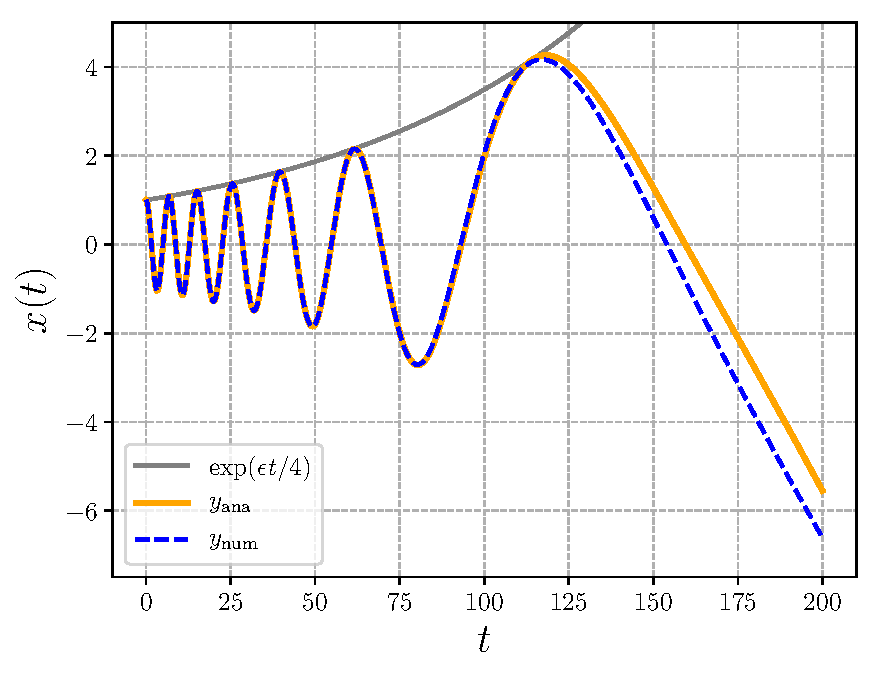
\includegraphics[width=0.75\textwidth]{./plots/pdf/strogatz-wk18.pdf}
	\caption{Solving eqn. \ref{eqn:wk18-spring-eqn} numerically and plotting eqn. \ref{eqn:wk18-spring-wkb} subject to the constraints given by eqns. \ref{eqn:wk18-spring-ic}.}
	\label{fig:strogatz-wk18}
\end{figure}







